%%%%%%%%%%%%%%%%%%%%%%%%%%%%%%%%%%%%%%%%%%%%%%%%%%%%%%%%%%%%%%%%%%%
%                                                                 %
%                            CHAPTER THREE                          %
%                                                                 %
%%%%%%%%%%%%%%%%%%%%%%%%%%%%%%%%%%%%%%%%%%%%%%%%%%%%%%%%%%%%%%%%%%%
\chapter{System Overview} \label{sec:system}

As stated in chapter 2, this thesis is an extension and modification of OASIS. The previous iteration of the user interface employed a 'drag-and-drop' method of introducing new elements. This chapter will explain in detail the processing entailed before recognizing the user's input. First, I will discuss where and how this work modifies the OASIS pipeline. The next section contains a detailed overview of strokes, the processing of those strokes, and extraction of useful metrics from them. Next, we cover actions available to the user in the sketching interface, such as creating walls, windows, and deleting previous objects. The final section consists of implementation elements, and its similarities and differences compared to OASIS.

\section{OASIS Pipeline}
In order to understand where this work improves OASIS, first I must discuss the pipeline OASIS follows to create new models. Figure \ref{fig:oasispipeline} illustrates the steps to completion from a user design to a finalized rendering. First, a user sketches a top-down 2D design of a room using the sketching interface. Users can then drag and drop walls, windows, and furniture onto a canvas. The placements and angles of furniture, the cardinal direction of the room, as well as its location in the world may be edited. Afterwards, the objects are converted into a primitives file which is interpreted by the physical sketch interpretation algorithm. This primitives file contains data about the attributes of walls and furniture, as well as room configurations. The physical sketch interpretation algorithm automatically interprets the sketch and exports it as a watertight triangle mesh  \cite{cutler2009inferring}. This mesh is rendered without lighting effects and simply confirms that the user's intentions were adequately interpreted into 3D from their 2D sketch. From any of their created meshes, users may create a simulation on the task manager page. Tasks may be edited with dates, times of day, timezones, and weather effects. After receiving a user-configured task, our server creates image textures based on the attributes set by the user. These textures are then used to map onto a finalized rendering shown to the user. \\

\begin{figure}[ht]
\centering
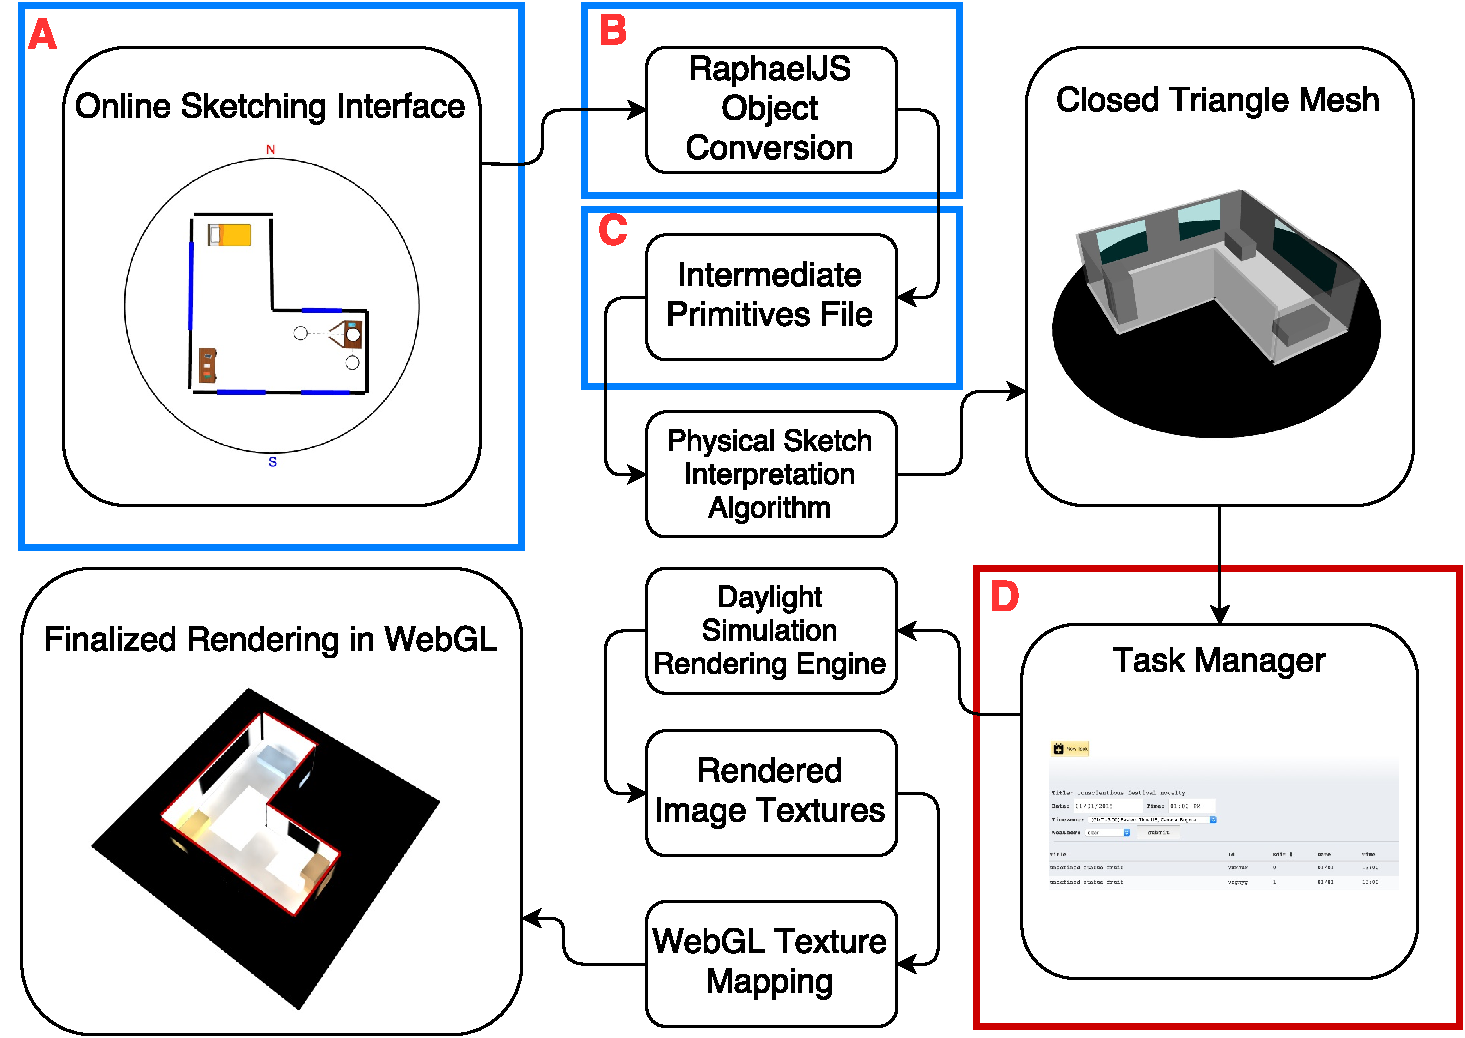
\includegraphics[width=\textwidth]{OASISpipeline2}
\caption[OASIS pipeline diagram]{Above is a diagram of the OASIS pipeline. Author's primary contributions are boxed in blue. Previous work is boxed in red.}
\label{fig:oasispipeline}
\end{figure}

In Figure \ref{fig:oasispipeline}, the boxes highlight which areas of OASIS I directly contributed to. The main contributions of this thesis to OASIS are the improvements to the online sketching interface, the RaphaelJS object conversion, and the modification of the intermediate primitives file. \\

\section{System Pipeline}
The system pipeline illustrated in Figure \ref{fig:systempipeline} outlines the primary stages of this thesis. Comparing to Figure \ref{fig:oasispipeline}, Figure \ref{fig:systempipeline} would belong between Figure \ref{fig:systempipeline}A and B, as shown in Figure \ref{fig:middlepipeline}. Improvements are also made to both the sketching interface and object conversion pipeline steps, which will both be discussed later in this chapter.

\begin{figure}[ht]
\centering
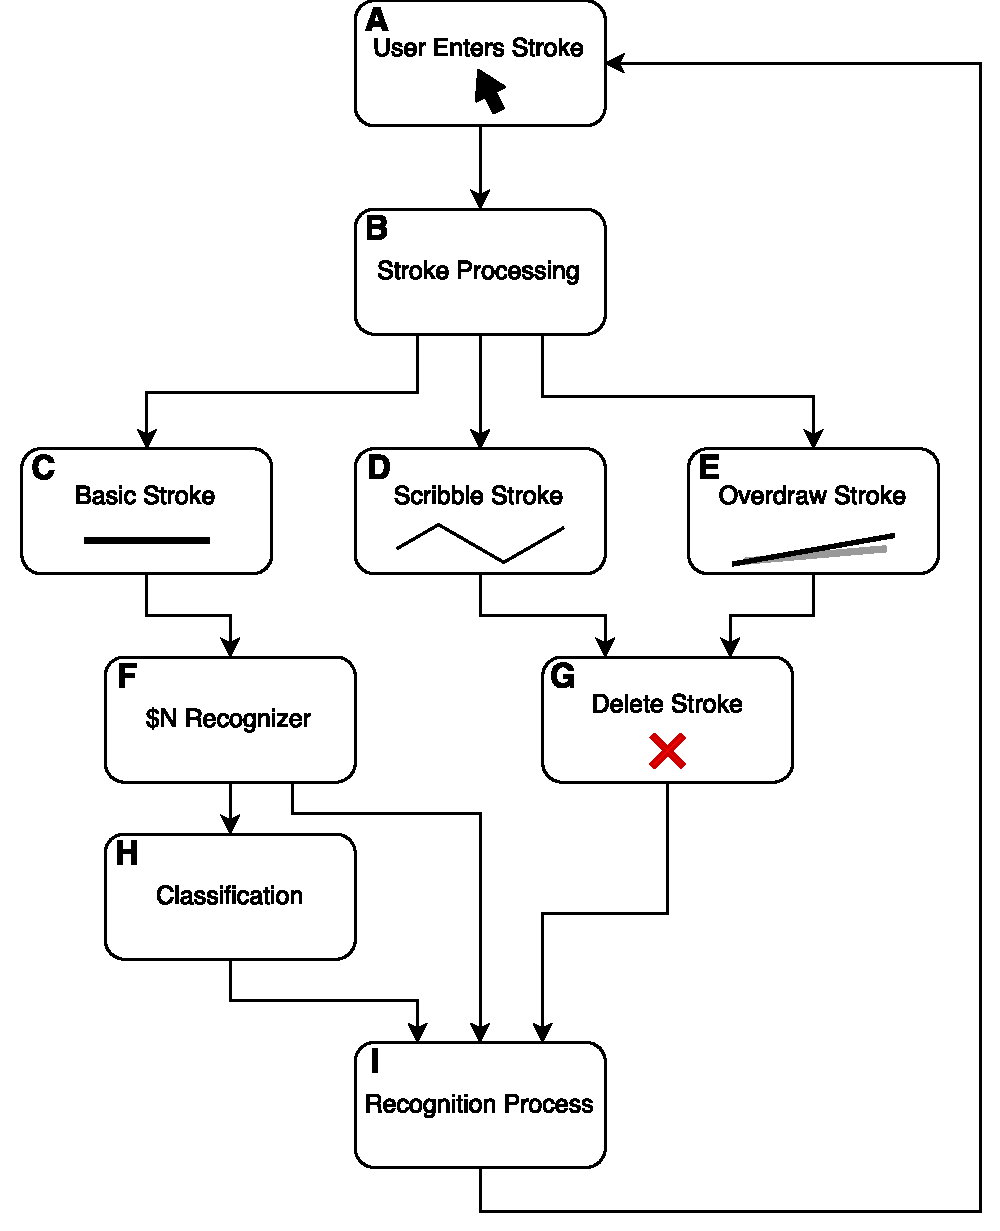
\includegraphics[width=.75\textwidth]{pipeline}
\caption[Sketching interface system pipeline diagram]{Above is a diagram of the system pipeline. This pipeline is contained within the stage represented by \ref{fig:middlepipeline}-A}
\label{fig:systempipeline}
\end{figure}

First, the system accepts a stroke, processes them into a standardized form, and create new attributes about the stroke. These steps are necessary to ensure accuracy when comparing different strokes. Afterwards, we identify the type of stroke based on properties calculated in the previous step. If the stroke is determined to be a scribble or overdraw, the system compares it against other strokes to determine if a deletion is necessary. If not, it is treated as a normal line segment or wall, and the system proceeds onto the recognition phase.  \\

\begin{figure}[ht]
\centering
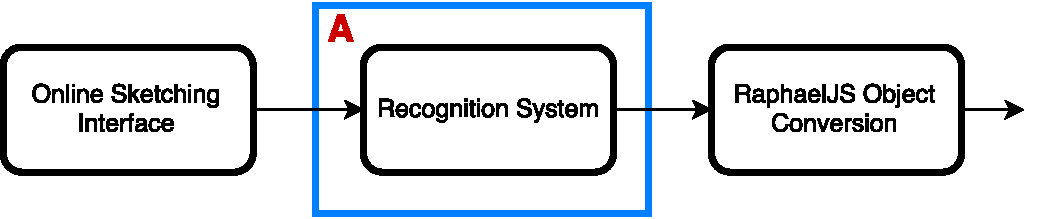
\includegraphics[width=\textwidth]{middle}
\caption[System pipeline diagram]{Above is the placement within the OASIS pipeline of the recognition system in which a majority of this work is contained.}
\label{fig:middlepipeline}
\end{figure}

If the stroke is determined to be a basic stroke after processing, it is fed into a the \$N recognizer to check if it similar to one of the template letters. If so, it will be used to reclassify an object according to the letter drawn. If not, it is treated as a normal line segment or wall and continues to the recognition phase. In the recognition phase, the system reevaluates the context of the set of strokes it has been given. The system will recognize any objects, fit an appropriate shape to them, display it to the user, and classify it under an object template.

\section{Stroke Processing}
\label{sec:strokeproc}

A point is defined as single pair of x and y coordinates. A stroke is a series of points on a canvas, and is the one of the most basic foundation data types in this system. To create a stroke, the user simply clicks anywhere on the interface, and moves their mouse to any other point on the interface without moving outside the boundaries. The system automatically records coordinates every time the mouse moves, creating a sequence of points. When the user releases his/her click, the points are converted into a stroke. In this section, I will review the processing done to these to simple points to interpret the user's intent.

\subsection{Stroke Resampling}
\label{sec:resample}

\begin{algorithm}
\caption[Pseudocode for resampling]{Psuedocode detailing resampling of a stroke}
\label{alg:resampling}
\begin{algorithmic}[1]
\Function{Resample}{points, numPoints, numDivisions}
\State $i \gets  PathLength(points) / (numDivisions -1)$
\State $d \gets $ 0
\State $resampled \gets $ [ ]
\For{$i = 0 \to numPoints$ }
    \State $m \gets  distance(point_{i-1}, point_i)$
    \If{$d+m < i$}
        \State $px \gets point_{i-1}.x + ((i-d)/m * (points_i.x - points_{i-1}.x))$ 
        \State $py \gets point_{i-1}.y + ((i-d)/m * (points_i.y - points_{i-1}.y))$ 
        \State $resampled \gets (px, py)$
        \State \textbf{insert} $(px,py)$ \textbf{in} points \textbf{at} i
    \Else
        \State $d = d+m$
    \EndIf
\EndFor
\State \textbf{return} $resampled$
\EndFunction
\end{algorithmic}
\end{algorithm}

After recording the raw coordinates of a stroke from the user, the first process required is resampling the stroke. Since a stroke is list of x and y coordinates, it is actually a series of short line segmenets. Unfortunately, due to differences in computer processing and human drawing speeds, these line segments may vary in length. The main purposes of resampling are to eliminate the inequality created by differences in speed when drawing strokes, and to remove clumping of points commonly created around corners. The inequality of the spacing between points of the line affects the scoring algorithms that rely on weighting metrics between all points equally. Algorithm \ref{alg:resampling} outlines the process to resample any number of points to \emph{numDivision} number of points. The algorithm finds the appropriate number of points, and the distance between each one such that they are all equidistant to their neighbors. There must a point every \emph{distance} length away, so we follow the stroke's path , point by point, creating a new point every time that threshold is crossed. At the end, there will exist exactly the number of points specified with equal distances between them. There is one flaw to this algorithm: it creates points that were not drawn by the user, and therefore the new set of points may not truly represent the user's original line. However, if the number of divisions is sufficiently high enough, the newly created set of points is a good approximation of the initial stroke. The average number of points per 150 pixels is approximately 30, and after resampling is the \emph{numDivision} number of points. I currently use 24 points per 150 pixels, through usage of the program I have found that using this number both generally lowers the number of points, and keeps a high degree of similarity to the user's original sketch.\\

Another possible method of resampling the line is to fit curvature of the line better. To accomplish this, extraneous points are removed from straight edges, and points are added to better define edges and curves. While this creates a better fitting line to the user's original input, the main purpose of fitting a line to the curvature is to lower the total number of points while retaining the shape of the line. However, my primary purpose of resampling the lines is to retain accuracy of our scoring algorithms by ensuring each point will have equal influence over the scoring of strokes or shapes.

\subsection{Line of Best Fit}
\label{sec:bestfit}
Since strokes contain many data points, it becomes very costly and difficult to draw comparisons between them. In cases where the strokes are perfectly straight lines, stroke comparison is simple. Properties such as angles and intersections between two or more lines are straightforward to calculate. Since not all strokes created are straight lines, it can be difficult to measure such attributes. In order to compare strokes, I have chosen to compute a linear line of best fit to generalize properties about a stroke. This reduces all strokes to straight lines, simplifying the process of comparing them. Treating the points of a stroke as scatter plot, a line of best fit will describe a set of properties that best fit the stroke. These properties include the slope, y-intercept, and the $r^2$ value. The slope determines the steepness of the line of best fit, the y-intercept controls the translation of that line, and the $r^2$ value represents how well the line fits the stroke's points. I used a least squares method to find my line for best fit, identifying the line with the least squared difference between it and each of the points in the stroke.

\subsection{LengthRatio}
\label{sec:lengthratio}
%definition of a stroke
%resampling
%length ratio, scribble

An important metric of a stroke is the line length to path length, or the \textit{LengthRatio}. The line length is the Euclidean distance from the first point to the last point. The path length is the summation of every line segment contained within the stroke. One useage of this metric is to determine if a user has drawn a line sufficiently close enough to a straight line. Since it is incredibly difficult to draw a perfectly straight line, I recognize when a user's stroke is close enough to a straight line, and fix it accordingly, as shown in Figure \ref{fig:walls}B-C. The equations for the calculation of the \textit{LengthRatio} are described below.

\begin{equation}
\label{equ:ratio1}
LineLength = distance(point_{0}, point_{n})
\end{equation}

\begin{equation}
\label{equ:ratio2}
PathLength = \sum_{i=0}^{n-1} distance(point_{i}, point_{i+1})
\end{equation}

\begin{equation}
\label{equ:ratio3}
LengthRatio = \dfrac{LineLength}{PathLength}
\end{equation}

Essentially, as the \textit{LengthRatio} approaches 1, the closer a stroke is to a perfectly straight line. Through some basic testing, I've determined .95 to be a reasonable cutoff for fixing crooked paths. \\

The same ratio is also used to determine strokes that are not definitely not straight lines, or `scribbles`. Scribbles are lines that are haphazard and random. To detect a scribble, the \textit{LengthRatio} is used, but with a different cutoff. The minimum \textit{LengthRatio} to be a line is .7, and any strokes under that are determined to be scribbles. 

% A very similar ratio is also used to determine strokes that are not definitely not straight lines, or `scribbles`. Scribbles are lines that are too haphazard and random. To detect a scribble, a \textit{AverageLengthRatio} is calculated every \emph{m} points, and averaged, as shown in Equation \ref{equ:ratio4}. A scribble typically has abrupt changes in direction, leading to a very high average \textit{LengthRatio}. An \textit{AverageLengthRatio} is used instead of an overall \textit{LengthRatio} in order to avoid capturing strokes such as a curve, which has a relatively high \textit{LengthRatio} compared to a straight line but a low \textit{AverageLengthRatio} compared to a scribble. The purpose of recognizing a straight line from a scribble is to delete previous strokes, which will be detailed further in the next section.

\section{Sketching Interface Actions}

In this section, we will discuss the features and actions available to the user to create and edit their designs. Since one goal was to preserve the simplicity of drawing, not many extraneous buttons or menu options were added. I did not want the user to feel pressured to remember hotkey combinations or highly specialized methods to perform certain actions. At minimum, the proposed new sketching interface has all the features of the previous system, plus added flexibility and ease of use.

\subsection{Walls and Windows}

As described earlier in Section \ref{sec:strokeproc}, a stroke is created on the new interface by clicking on the interface and dragging to another location. An example of how a user would create a wall is outlined in Figure \ref{fig:walls}A-C. At a base level, all strokes are considered walls until recognized or classified as otherwise. The next chapter will cover the classification and recognition of objects in further detail.

\begin{figure}[ht]
\centering
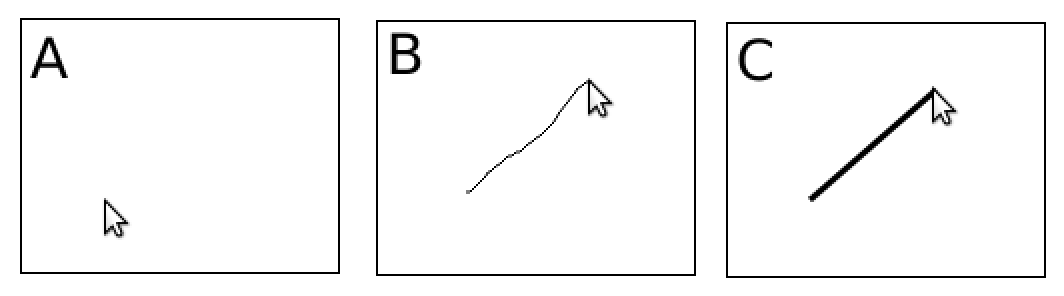
\includegraphics[width=\textwidth]{walls}
\caption[How to create a wall using the sketching interface]{How to create a wall using the sketching interface.}
\label{fig:walls}
\end{figure}

The new sketching interface mimics how one would draw with pencil and paper, without the need to click on buttons or referring to toolbar. As demonstrated in Figure \ref{fig:walls}, the strokes will snap to a straight line if the LengthRatio has crossed a threshold of .95. This is achieved by replacing the previously recorded points with a segement of the line of best fit. This is determined by finding the points on the line of best closest to the first and last point created by the user. Given that most physical walls are straight, and that it would be difficult to straighten lines without any tools on the interface, it made sense to automatically fix slightly crooked walls. Overall, it was a change that resulted in much cleaner looking designs. \\

Windows can be created just as seamlessly as walls in the new interface. Windows must be attached to a wall, and cannot be longer than the wall it belongs to. As shown in Figure \ref{fig:windows}-A, a user mouses over a wall, changing the wall's color to red. Next, the user clicks on the wall and drags the wall to the desired length, as illustrated in Figure \ref{fig:windows}-B. Finally, to create the window, the user releases his or her mouse click, snapping the window to the wall, as depicted by Figure \ref{fig:windows}-C.

\begin{figure}[ht]
\centering
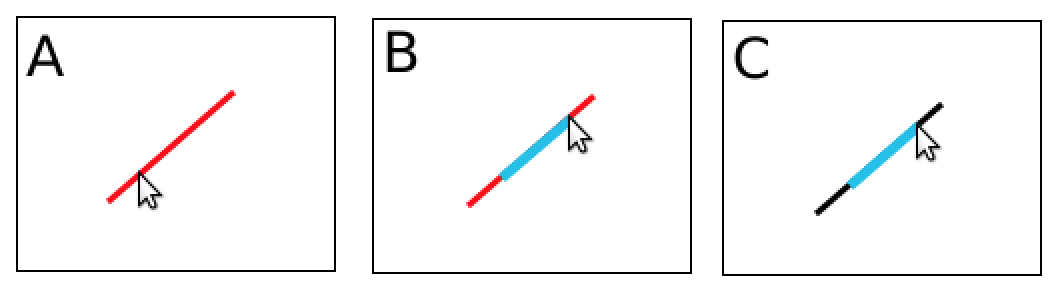
\includegraphics[width=\textwidth]{windows}
\caption[How to create a window using the sketching interface]{How to create a window using the sketching interface.}
\label{fig:windows}
\end{figure}

The window snapping algorithm uses the best fit line of the wall it is attached to. The user chooses the length of the window by designating a start and end point, and the the slope of the window is determined by the slope of the line it is attached to. In order to allow for flexibility, walls do not need to be dragged in the exact direction or orientation to snap to the wall. The proposed window can be dragged into any angle, and even beyond the length of the wall. However, should a user mistakenly enter the window creation process, he/she can drag the cursor such that it creates a perpendicular angle with the wall, ensuring that the window does not get created at all. Regardless of how long the wall is dragged, it will always snap up to a maximum of 5 percent away from the end, towards the center of the wall. This is to allow some space for the window, and to avoid some bugs that have been discovered with windows attached walls that are equally as long.

\subsection{Deleting Strokes}

Should the user make the inevitable mistake, the ability to delete strokes would be a welcomed feature. Keeping in the spirit of design without using a toolbar, users can 'scribble' or draw over their previous strokes to delete or modify them. The act of modifying a stroke is very similar to the previously described actions. \\

It is simple to scribble out a previously drawn stroke. As shown in Figure \ref{fig:scribble}, a user find the stroke he/she wants to remove, then sketches a random stroke resembling a scribble over the chosen stroke, and both strokes disappear.

\begin{figure}[ht]
\centering
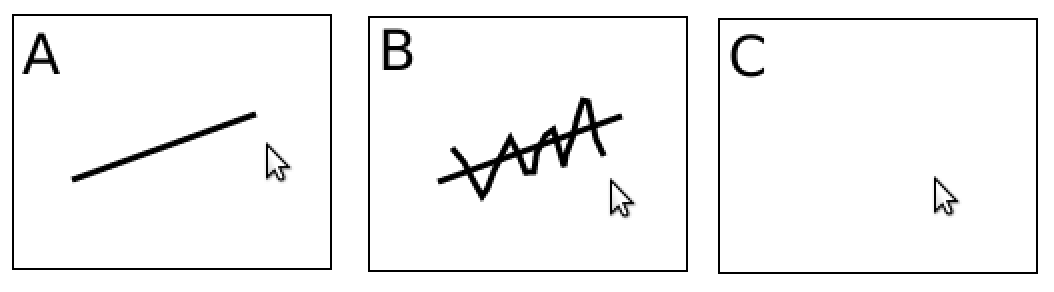
\includegraphics[width=\textwidth]{scribble}
\caption[How to delete a stroke by scribbling]{How to delete a stroke by scribbling.}
\label{fig:scribble}
\end{figure}

As mentioned before in Section \ref{sec:lengthratio}, if the LengthRatio is under .7, a stroke is classified as a scribble. If a stroke is detected as a scribble, we search for strokes whose points are near those of the scribble. If another stroke is in the immediate area, then both strokes are removed from the sketch. However, the strokes do continue to remain in the system, allowing for the possibility of an undo feature in the future.\\

To draw over a stroke, a similar process to scribbling is employed. First, the user finds a stroke he/she would like removed, as exhibited in Figure \ref{fig:scribble}. The stroke is currently only greyed out in the image and not the application itself. However, it could be a feature for development in the future, since the viewing of previous strokes may visually assist the user when designing. Next, the user draws a line with similar angle, length, and positioning to the undesired stroke. Finally, the previous stroke is removed and the new stroke remains.

\begin{figure}[ht]
\centering
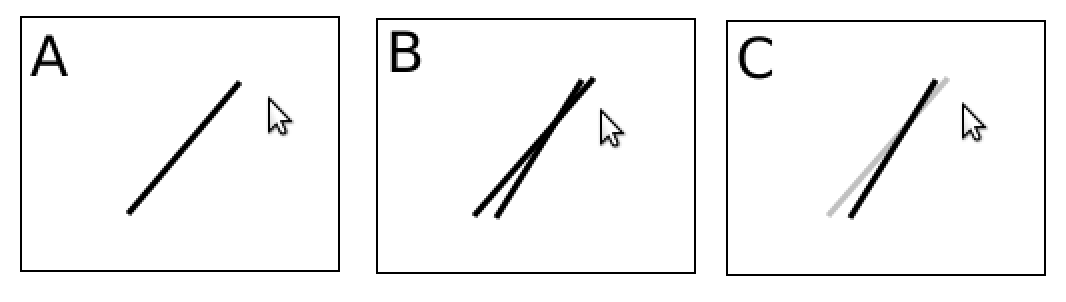
\includegraphics[width=\textwidth]{overdraw}
\caption[How to overdraw a previous stroke]{How to draw over a previous stroke. The removed stroke is greyed out only for this figure, to help visualize the removal.}
\label{fig:overdraw}
\end{figure}

The process behind overdrawing a stroke is also similar to that of scribbling. However, instead of checking for the presence of a scribble, I check for the distance between the overdraw stroke and every other stroke. The distance between strokes is calculated between the centers of the strokes. We compare the stroke's properties taken from its line of best fit to its closest neighbors, which are only strokes whose centers are within half its \textit{pathLength} away from its own center. If any other strokes are similar enough in length and angle, we delete the previous stroke and allow the newly drawn stroke to remain. If no strokes fit the criteria, then the stroke is treated as a normal wall. \\

Previously, a two dimensional grid was used to store stroke information and compare location data. While it is more computationally efficient with extremely high numbers of strokes, the overhead and complexity to maintain such a data structure with low numbers of strokes far outweighed the benefits. After testing with moderately complex models with 20-40 strokes, it was determined that the use of a spatial data structure was either the same or slower speed than checking against all other strokes. Should models become more complex in the future, this data structure could be revisited. However, in its current iteration, there is not enough data in an average model to warrant the use of a spatial structure.

\subsection{Cardinal Direction}

With the production of a new sketching interface, it was necessary to consider a new method of indicating the cardinal direction, such as north or south. The previous implementation was a movable ring surrounding the design area. However, ring would be an inefficient use of space with a rectangular sketching area. The proposed idea is a small north arrow on the canvas indicating the direction of north. The arrow will rotate away from the center every time it is adjusted. Users will be able to easily move the indicator without clicking on a toolbar. The equation used to calculate the angle away from the center given a point and a center is shown in Equation \ref{equ:anglecenternorth}.

\begin{equation}
\label{equ:anglecenternorth}
Angle = \tan{(\dfrac{point_y - center_y}{point_x - center_x})}
\end{equation}

\begin{figure}[ht]
\centering
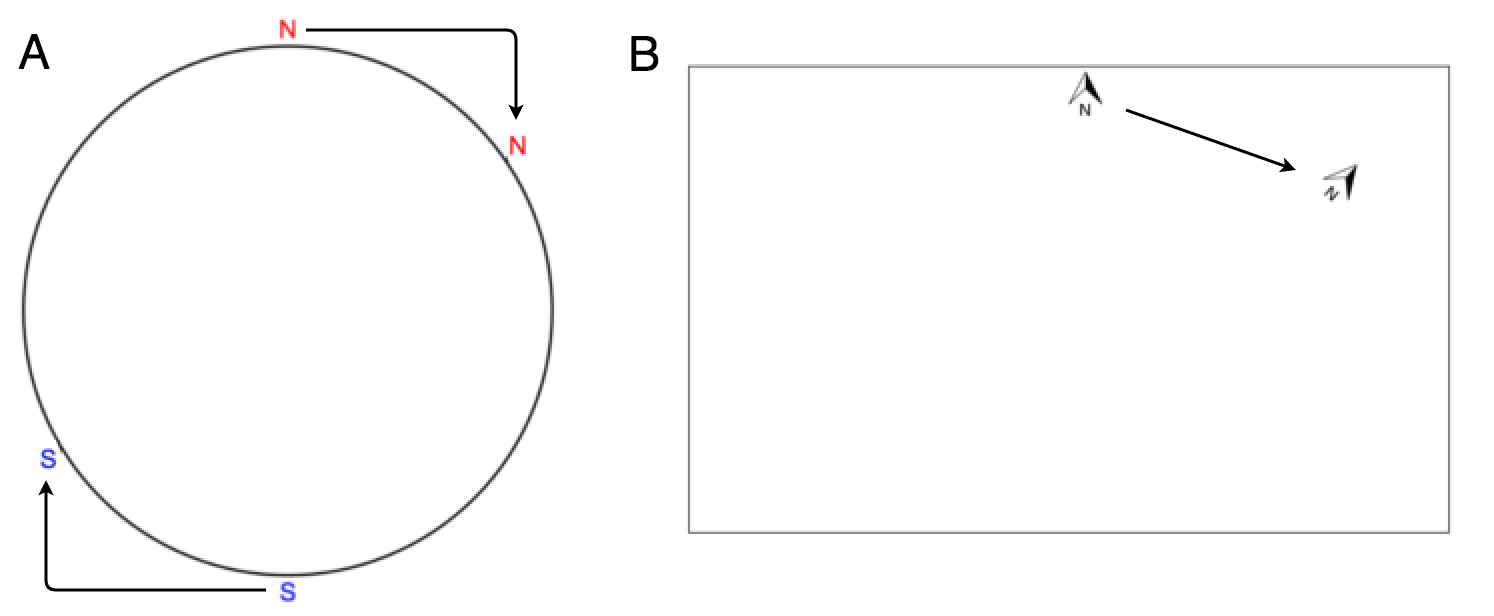
\includegraphics[width=\textwidth]{compass}
\caption[Comparison of cardinal direction changes between interfaces]{An illustration between the two methods of changing cardinal direction in each interface.}
\label{fig:compass}
\end{figure}

\section{System Design and Implementation Details}

In this section, I will give a brief overview of system design choices that are not a direct part of the sketching interface itself. While they do not necessarily directly affect the user, it is important to understand these design choices and their impacts on the user and the future of OASIS.

\subsection{Intermediate Primitives File}

Due to the possible additional complexity of walls, a decision was made to move away from the previous primitives file format. The previous format was designed to recognize physical objects placed on a table, with small numbers of primitives, and record data such as position and orientation. However, in the new interface, with walls and strokes capable of containing over 100 points (and thus over 100 wall segments), the amount of data stored needed to be simpler to store and access. The new proposed intermediate primitives file format will be in Javascript Object Notation (JSON). JSON is a language independent, lightweight, data-interchange format that is easy for humans to read and widely generated and parsed by many operating systems and applications \cite{json}. JSON is often used to transmit data from servers to applications and consists of attribute/value pairs. Given its widespread use, it would allow the data collected in this application more accessible to other programs and make integration with future features simpler. Also, being a standardized format will require less specialized knowledge to understand. Moving forward, the switch to the JSON file format will make the application more accessible for feature development and more manageable to maintain. 

% \subsection{Inclusion of both sketching interfaces}

% Currently, when a user creates a new model, the user has an option to design with either the previous user interface or the new sketching interface. An image of the menu is displayed in Figure \ref{fig:choice}.

% \begin{figure}[ht]
% \centering
% 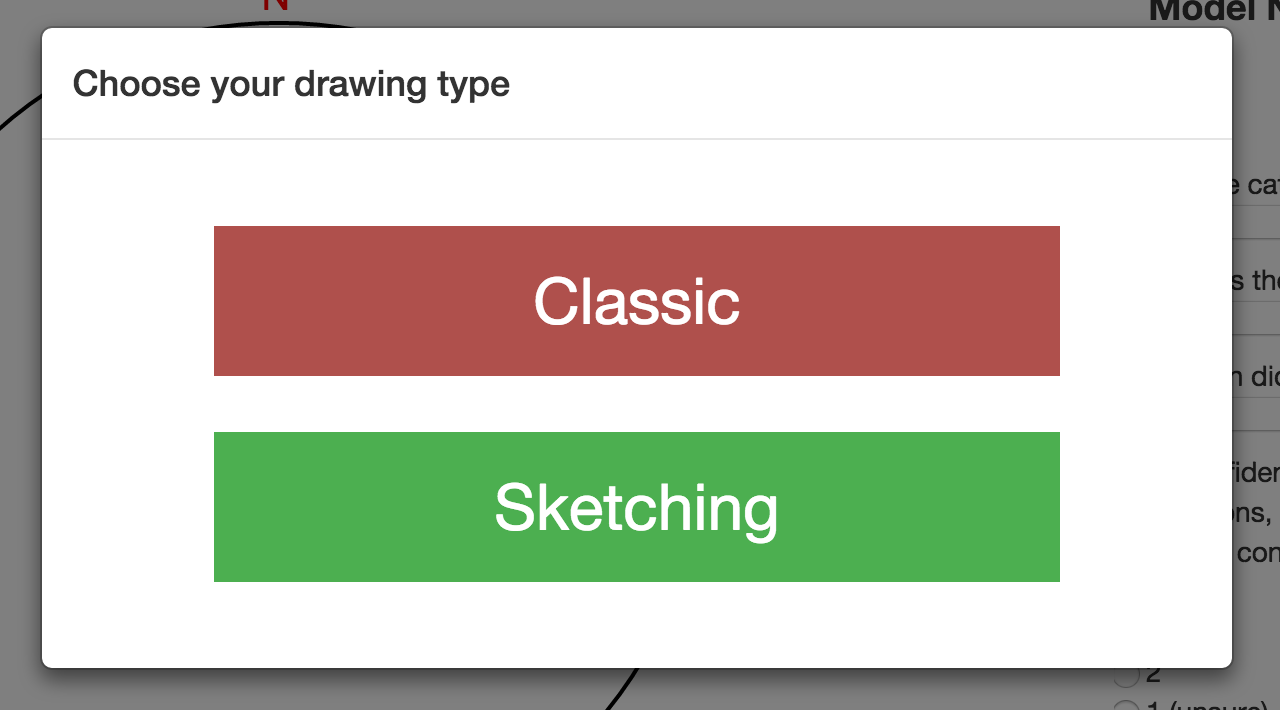
\includegraphics[width=.75\textwidth]{choice}
% \caption[Image of choice between interfaces]{Upon choosing to design a new model, the user may choose between the previous interface or the new one.}
% \label{fig:choice}
% \end{figure}

% The reasoning behind the choice to allow the user to choose his/her method of sketching was to support the decision of the user of the more comfortable interface. While I would be delighted if every single user thought this new sketching interface was undeniably better than the previous one, it is unlikely to true. In a topic as arbitrary as design methodology, every user has his/her unique preferences, and it is not possible to be perfect in every scenario. I believe that it is in the application's best interest to allow each user to select his or her preference.

\subsection{Technologies}

Being an extension and modification of OASIS, it is logical that the two have technologies and frameworks in common. Both applications are built primarily on Javascript, and both rely heavily on the RapahelJS \cite{raphaeljs} framework. RaphaelJS is a vector graphics Javascript framework that supports most major web browsers. RaphaelJS is used to create all the sketching elements, including walls, windows, and furniture. It allowed for the easy creation and manipulation of lines and shapes created by the user. FreeTransform \cite{freetransform}, which is an extension of RaphaelJS, is used for the rearrangement of objects in the sketching interface. Due to the method of storing positional values by RaphaelJS, moving an object multiple times is complex. Both RaphaelJS and its extension, FreeTransform were instrumental in the development of this work.

%talk about the new wallfile
%talk about choice of sketching
%technologies used

\section{Chapter Summary}

This chapter reviewed the pipeline of OASIS and where  this work contributed within that process. An overview of strokes, processing of those strokes, and stroke metrics were provided. Next, I presented the elements and actions available within the sketching interface itself. Afterwards, I discussed some of the design choices behind the development of this thesis and its impact on the application. The next chapter examines in further detail the logic behind recognition and classification of objects in the sketching interface.